\documentclass[twoside]{book}

% Packages required by doxygen
\usepackage{fixltx2e}
\usepackage{calc}
\usepackage{doxygen}
\usepackage[export]{adjustbox} % also loads graphicx
\usepackage{graphicx}
\usepackage[utf8]{inputenc}
\usepackage{makeidx}
\usepackage{multicol}
\usepackage{multirow}
\PassOptionsToPackage{warn}{textcomp}
\usepackage{textcomp}
\usepackage[nointegrals]{wasysym}
\usepackage[table]{xcolor}

% Font selection
\usepackage[T1]{fontenc}
\usepackage[scaled=.90]{helvet}
\usepackage{courier}
\usepackage{amssymb}
\usepackage{sectsty}
\renewcommand{\familydefault}{\sfdefault}
\allsectionsfont{%
  \fontseries{bc}\selectfont%
  \color{darkgray}%
}
\renewcommand{\DoxyLabelFont}{%
  \fontseries{bc}\selectfont%
  \color{darkgray}%
}
\newcommand{\+}{\discretionary{\mbox{\scriptsize$\hookleftarrow$}}{}{}}

% Page & text layout
\usepackage{geometry}
\geometry{%
  a4paper,%
  top=2.5cm,%
  bottom=2.5cm,%
  left=2.5cm,%
  right=2.5cm%
}
\tolerance=750
\hfuzz=15pt
\hbadness=750
\setlength{\emergencystretch}{15pt}
\setlength{\parindent}{0cm}
\setlength{\parskip}{3ex plus 2ex minus 2ex}
\makeatletter
\renewcommand{\paragraph}{%
  \@startsection{paragraph}{4}{0ex}{-1.0ex}{1.0ex}{%
    \normalfont\normalsize\bfseries\SS@parafont%
  }%
}
\renewcommand{\subparagraph}{%
  \@startsection{subparagraph}{5}{0ex}{-1.0ex}{1.0ex}{%
    \normalfont\normalsize\bfseries\SS@subparafont%
  }%
}
\makeatother

% Headers & footers
\usepackage{fancyhdr}
\pagestyle{fancyplain}
\fancyhead[LE]{\fancyplain{}{\bfseries\thepage}}
\fancyhead[CE]{\fancyplain{}{}}
\fancyhead[RE]{\fancyplain{}{\bfseries\leftmark}}
\fancyhead[LO]{\fancyplain{}{\bfseries\rightmark}}
\fancyhead[CO]{\fancyplain{}{}}
\fancyhead[RO]{\fancyplain{}{\bfseries\thepage}}
\fancyfoot[LE]{\fancyplain{}{}}
\fancyfoot[CE]{\fancyplain{}{}}
\fancyfoot[RE]{\fancyplain{}{\bfseries\scriptsize Generated by Doxygen }}
\fancyfoot[LO]{\fancyplain{}{\bfseries\scriptsize Generated by Doxygen }}
\fancyfoot[CO]{\fancyplain{}{}}
\fancyfoot[RO]{\fancyplain{}{}}
\renewcommand{\footrulewidth}{0.4pt}
\renewcommand{\chaptermark}[1]{%
  \markboth{#1}{}%
}
\renewcommand{\sectionmark}[1]{%
  \markright{\thesection\ #1}%
}

% Indices & bibliography
\usepackage{natbib}
\usepackage[titles]{tocloft}
\setcounter{tocdepth}{3}
\setcounter{secnumdepth}{5}
\makeindex

% Hyperlinks (required, but should be loaded last)
\usepackage{ifpdf}
\ifpdf
  \usepackage[pdftex,pagebackref=true]{hyperref}
\else
  \usepackage[ps2pdf,pagebackref=true]{hyperref}
\fi
\hypersetup{%
  colorlinks=true,%
  linkcolor=blue,%
  citecolor=blue,%
  unicode%
}

% Custom commands
\newcommand{\clearemptydoublepage}{%
  \newpage{\pagestyle{empty}\cleardoublepage}%
}

\usepackage{caption}
\captionsetup{labelsep=space,justification=centering,font={bf},singlelinecheck=off,skip=4pt,position=top}

%===== C O N T E N T S =====

\begin{document}

% Titlepage & ToC
\hypersetup{pageanchor=false,
             bookmarksnumbered=true,
             pdfencoding=unicode
            }
\pagenumbering{roman}
\begin{titlepage}
\vspace*{7cm}
\begin{center}%
{\Large My Project }\\
\vspace*{1cm}
{\large Generated by Doxygen 1.8.11}\\
\end{center}
\end{titlepage}
\clearemptydoublepage
\tableofcontents
\clearemptydoublepage
\pagenumbering{arabic}
\hypersetup{pageanchor=true}

%--- Begin generated contents ---
\chapter{Hierarchical Index}
\section{Class Hierarchy}
This inheritance list is sorted roughly, but not completely, alphabetically\+:\begin{DoxyCompactList}
\item \contentsline{section}{Staff}{\pageref{class_staff}}{}
\begin{DoxyCompactList}
\item \contentsline{section}{Faculty}{\pageref{class_faculty}}{}
\item \contentsline{section}{Officer}{\pageref{class_officer}}{}
\item \contentsline{section}{Typist}{\pageref{class_typist}}{}
\begin{DoxyCompactList}
\item \contentsline{section}{Casual}{\pageref{class_casual}}{}
\item \contentsline{section}{Permanent}{\pageref{class_permanent}}{}
\end{DoxyCompactList}
\end{DoxyCompactList}
\end{DoxyCompactList}

\chapter{Class Index}
\section{Class List}
Here are the classes, structs, unions and interfaces with brief descriptions\+:\begin{DoxyCompactList}
\item\contentsline{section}{\hyperlink{class_casual}{Casual} }{\pageref{class_casual}}{}
\item\contentsline{section}{\hyperlink{class_faculty}{Faculty} }{\pageref{class_faculty}}{}
\item\contentsline{section}{\hyperlink{class_officer}{Officer} }{\pageref{class_officer}}{}
\item\contentsline{section}{\hyperlink{class_permanent}{Permanent} }{\pageref{class_permanent}}{}
\item\contentsline{section}{\hyperlink{class_staff}{Staff} }{\pageref{class_staff}}{}
\item\contentsline{section}{\hyperlink{class_typist}{Typist} }{\pageref{class_typist}}{}
\end{DoxyCompactList}

\chapter{File Index}
\section{File List}
Here is a list of all files with brief descriptions\+:\begin{DoxyCompactList}
\item\contentsline{section}{\hyperlink{person_8cpp}{person.\+cpp} }{\pageref{person_8cpp}}{}
\end{DoxyCompactList}

\chapter{Class Documentation}
\hypertarget{class_casual}{}\section{Casual Class Reference}
\label{class_casual}\index{Casual@{Casual}}


Inheritance diagram for Casual\+:
\nopagebreak
\begin{figure}[H]
\begin{center}
\leavevmode
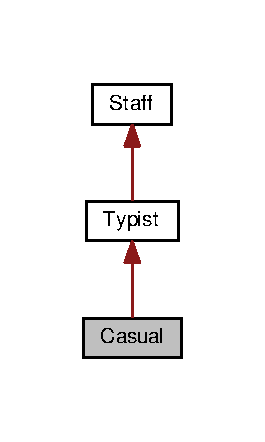
\includegraphics[width=127pt]{class_casual__inherit__graph}
\end{center}
\end{figure}


Collaboration diagram for Casual\+:
\nopagebreak
\begin{figure}[H]
\begin{center}
\leavevmode
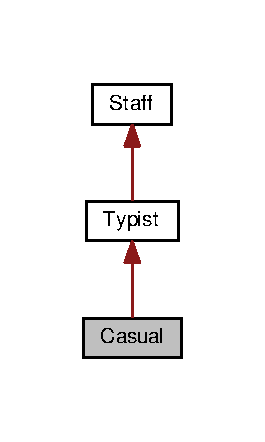
\includegraphics[width=127pt]{class_casual__coll__graph}
\end{center}
\end{figure}


The documentation for this class was generated from the following file\+:\begin{DoxyCompactItemize}
\item 
\hyperlink{inheritance_8cpp}{inheritance.\+cpp}\end{DoxyCompactItemize}

\hypertarget{class_faculty}{}\section{Faculty Class Reference}
\label{class_faculty}\index{Faculty@{Faculty}}


Inheritance diagram for Faculty\+:
\nopagebreak
\begin{figure}[H]
\begin{center}
\leavevmode
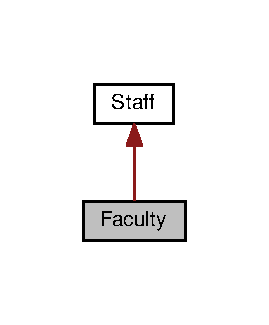
\includegraphics[width=129pt]{class_faculty__inherit__graph}
\end{center}
\end{figure}


Collaboration diagram for Faculty\+:
\nopagebreak
\begin{figure}[H]
\begin{center}
\leavevmode
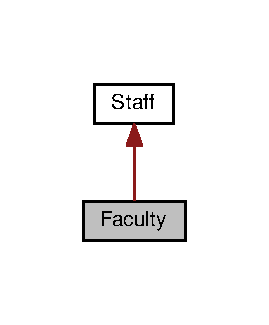
\includegraphics[width=129pt]{class_faculty__coll__graph}
\end{center}
\end{figure}


The documentation for this class was generated from the following file\+:\begin{DoxyCompactItemize}
\item 
\hyperlink{inheritance_8cpp}{inheritance.\+cpp}\end{DoxyCompactItemize}

\hypertarget{class_officer}{}\section{Officer Class Reference}
\label{class_officer}\index{Officer@{Officer}}


Inheritance diagram for Officer\+:
\nopagebreak
\begin{figure}[H]
\begin{center}
\leavevmode
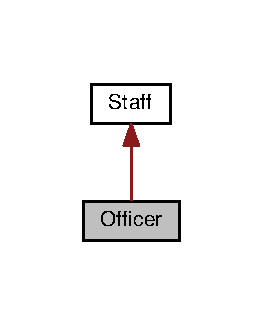
\includegraphics[width=126pt]{class_officer__inherit__graph}
\end{center}
\end{figure}


Collaboration diagram for Officer\+:
\nopagebreak
\begin{figure}[H]
\begin{center}
\leavevmode
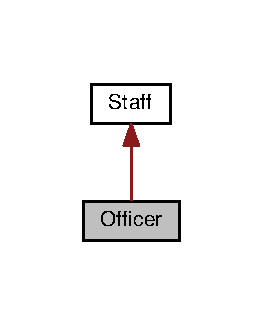
\includegraphics[width=126pt]{class_officer__coll__graph}
\end{center}
\end{figure}


The documentation for this class was generated from the following file\+:\begin{DoxyCompactItemize}
\item 
\hyperlink{inheritance_8cpp}{inheritance.\+cpp}\end{DoxyCompactItemize}

\hypertarget{class_permanent}{}\section{Permanent Class Reference}
\label{class_permanent}\index{Permanent@{Permanent}}


Inheritance diagram for Permanent\+:
\nopagebreak
\begin{figure}[H]
\begin{center}
\leavevmode
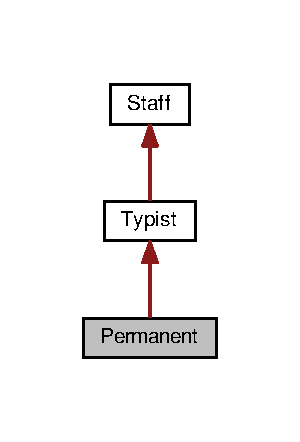
\includegraphics[width=144pt]{class_permanent__inherit__graph}
\end{center}
\end{figure}


Collaboration diagram for Permanent\+:
\nopagebreak
\begin{figure}[H]
\begin{center}
\leavevmode
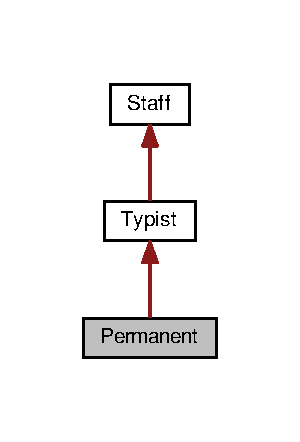
\includegraphics[width=144pt]{class_permanent__coll__graph}
\end{center}
\end{figure}


The documentation for this class was generated from the following file\+:\begin{DoxyCompactItemize}
\item 
\hyperlink{inheritance_8cpp}{inheritance.\+cpp}\end{DoxyCompactItemize}

\hypertarget{class_staff}{}\section{Staff Class Reference}
\label{class_staff}\index{Staff@{Staff}}


Inheritance diagram for Staff\+:
\nopagebreak
\begin{figure}[H]
\begin{center}
\leavevmode
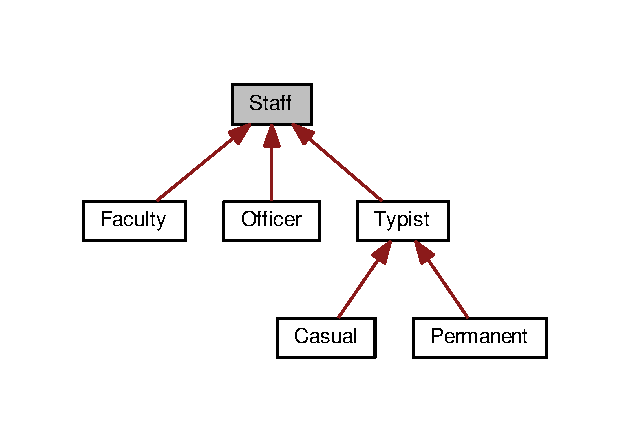
\includegraphics[width=303pt]{class_staff__inherit__graph}
\end{center}
\end{figure}


The documentation for this class was generated from the following file\+:\begin{DoxyCompactItemize}
\item 
\hyperlink{inheritance_8cpp}{inheritance.\+cpp}\end{DoxyCompactItemize}

\hypertarget{class_typist}{}\section{Typist Class Reference}
\label{class_typist}\index{Typist@{Typist}}


Inheritance diagram for Typist\+:
\nopagebreak
\begin{figure}[H]
\begin{center}
\leavevmode
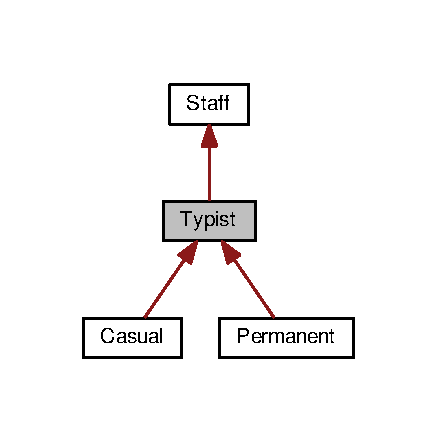
\includegraphics[width=210pt]{class_typist__inherit__graph}
\end{center}
\end{figure}


Collaboration diagram for Typist\+:
\nopagebreak
\begin{figure}[H]
\begin{center}
\leavevmode
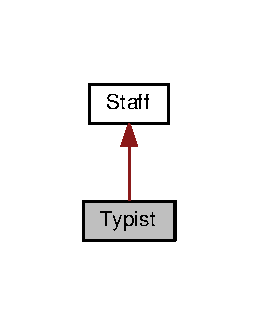
\includegraphics[width=124pt]{class_typist__coll__graph}
\end{center}
\end{figure}


The documentation for this class was generated from the following file\+:\begin{DoxyCompactItemize}
\item 
\hyperlink{inheritance_8cpp}{inheritance.\+cpp}\end{DoxyCompactItemize}

\chapter{File Documentation}
\hypertarget{inheritance_8cpp}{}\section{inheritance.\+cpp File Reference}
\label{inheritance_8cpp}\index{inheritance.\+cpp@{inheritance.\+cpp}}
{\ttfamily \#include $<$iostream$>$}\\*
{\ttfamily \#include $<$string$>$}\\*
Include dependency graph for inheritance.\+cpp\+:
\nopagebreak
\begin{figure}[H]
\begin{center}
\leavevmode
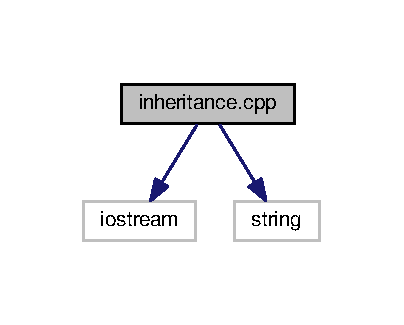
\includegraphics[width=194pt]{inheritance_8cpp__incl}
\end{center}
\end{figure}
\subsection*{Classes}
\begin{DoxyCompactItemize}
\item 
class \hyperlink{class_staff}{Staff}
\item 
class \hyperlink{class_faculty}{Faculty}
\item 
class \hyperlink{class_typist}{Typist}
\item 
class \hyperlink{class_officer}{Officer}
\item 
class \hyperlink{class_permanent}{Permanent}
\item 
class \hyperlink{class_casual}{Casual}
\end{DoxyCompactItemize}
\subsection*{Functions}
\begin{DoxyCompactItemize}
\item 
int \hyperlink{inheritance_8cpp_ae66f6b31b5ad750f1fe042a706a4e3d4}{main} ()
\end{DoxyCompactItemize}


\subsection{Function Documentation}
\index{inheritance.\+cpp@{inheritance.\+cpp}!main@{main}}
\index{main@{main}!inheritance.\+cpp@{inheritance.\+cpp}}
\subsubsection[{\texorpdfstring{main()}{main()}}]{\setlength{\rightskip}{0pt plus 5cm}int main (
\begin{DoxyParamCaption}
{}
\end{DoxyParamCaption}
)}\hypertarget{inheritance_8cpp_ae66f6b31b5ad750f1fe042a706a4e3d4}{}\label{inheritance_8cpp_ae66f6b31b5ad750f1fe042a706a4e3d4}

%--- End generated contents ---

% Index
\backmatter
\newpage
\phantomsection
\clearemptydoublepage
\addcontentsline{toc}{chapter}{Index}
\printindex

\end{document}
